\documentclass[11pt]{article}

\usepackage[margin=1in]{geometry}
\usepackage{graphicx}
\usepackage{hyperref}
\usepackage{amsmath}
\usepackage{array}
\usepackage{caption}
\usepackage{subcaption}

\title{\textbf{PromptLite-Seg: Lightweight Zero-Shot Prompted Segmentation on PASCAL VOC 2012}}
\author{ZhouYinLong-lab}
\date{\today}

\begin{document}
\maketitle

\begin{abstract}
PromptLite-Seg studies zero-shot prompted segmentation on PASCAL VOC 2012. Given a weak prompt consisting of a center point and a bounding box, the goal is to segment the target object without training on the benchmark. The project implements a simple center-color baseline and a stronger SAM-free robust superpixel method. The robust method uses prompt-induced foreground/background prototypes, box constraints, superpixel consensus, and lightweight morphology. On a 30-sample VOC 2012 validation subset, the robust method improves mean IoU from 0.5468 to 0.6031 and mean Dice from 0.6754 to 0.7277.
\end{abstract}

\section{Introduction}

Prompted segmentation has become a practical interface for general-purpose vision systems. Models such as the Segment Anything Model (SAM) demonstrate that segmentation can be controlled by points and boxes. However, large pretrained models may be expensive to run or difficult to reproduce in a lightweight course setting. This project therefore asks a complementary question: how far can a transparent, training-free prompted segmentation algorithm go on real benchmark images?

The task follows the course-design direction of zero-shot prompt segmentation. The benchmark is PASCAL VOC 2012. For each selected validation sample, the largest semantic object component is converted into a binary target mask. The prompt consists of a tight bounding box and an interior center point derived from the distance transform of the target mask.

\section{Method}

\subsection{Prompt Generation}

PASCAL VOC semantic masks provide foreground labels from 1 to 20 and background label 0. For each sample, PromptLite-Seg selects the largest connected foreground component as the target instance. The bounding box is the tight rectangle around this component. The point prompt is the pixel with maximum distance-transform value inside the component, which approximates a stable human center click.

\subsection{Center-Color Baseline}

The baseline estimates the target appearance from a small disk around the center point. Pixels inside the prompt box are segmented if their RGB distance to this median color prototype is below an adaptive Otsu threshold. Small components are removed, holes are filled, and the connected component nearest to the prompt point is retained.

\subsection{Robust Superpixel Prompt Segmentation}

The robust method first runs the center-color baseline to obtain a conservative foreground seed. It then oversegments the image into SLIC superpixels. Each superpixel is represented by mean Lab color and normalized spatial coordinates. Foreground prototypes are estimated from superpixels intersecting the center-point disk, while background prototypes are estimated from superpixels outside the prompt box and along the box border.

Each superpixel receives a foreground score based on its relative distance to foreground and background prototypes, combined with a weak spatial prior centered at the prompt point. The final mask is the union of the conservative color seed and superpixel consensus across slightly perturbed boxes, followed by morphology and point-connected component selection.

\section{Experimental Setup}

The experiment uses a compact subset of PASCAL VOC 2012 validation samples from the Hugging Face mirror \texttt{nateraw/pascal-voc-2012}. The subset contains 30 samples and 12 object classes. The evaluation reports Intersection over Union (IoU) and Dice score:

\[
\text{IoU} = \frac{|P \cap G|}{|P \cup G|}, \qquad
\text{Dice} = \frac{2|P \cap G|}{|P| + |G|}.
\]

The reproducible commands are:

\begin{verbatim}
python scripts/download_voc_subset.py --count 30
python scripts/run_experiment.py --max-samples 30
python scripts/analyze_results.py
\end{verbatim}

\section{Results}

\begin{table}[h]
\centering
\caption{Aggregate results on the 30-sample VOC 2012 subset.}
\begin{tabular}{lrrrr}
\hline
Method & Mean IoU & Std IoU & Mean Dice & Std Dice \\
\hline
Center-color baseline & 0.5468 & 0.2323 & 0.6754 & 0.2122 \\
Robust superpixel & 0.6031 & 0.2111 & 0.7277 & 0.1895 \\
\hline
\end{tabular}
\end{table}

The robust method improves mean IoU by 0.0562 absolute points and mean Dice by 0.0523. At the sample level, it wins on 23 samples, ties on 5 samples, and loses on only 2 samples relative to the center-color baseline.

\begin{figure}[h]
\centering
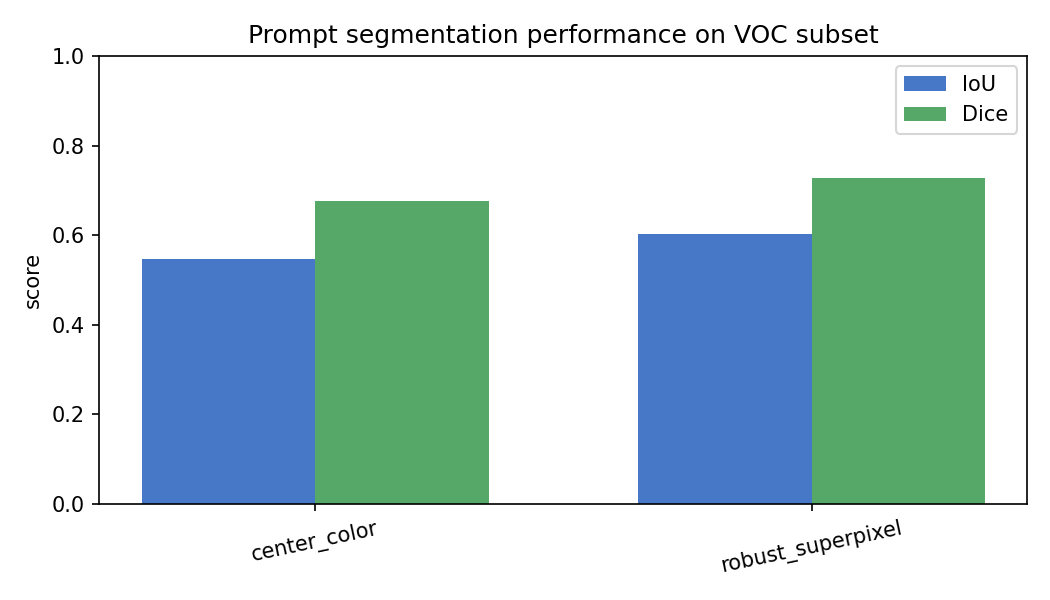
\includegraphics[width=0.72\linewidth]{../outputs/figures/metric_summary.png}
\caption{Aggregate IoU and Dice comparison.}
\end{figure}

\begin{figure}[h]
\centering
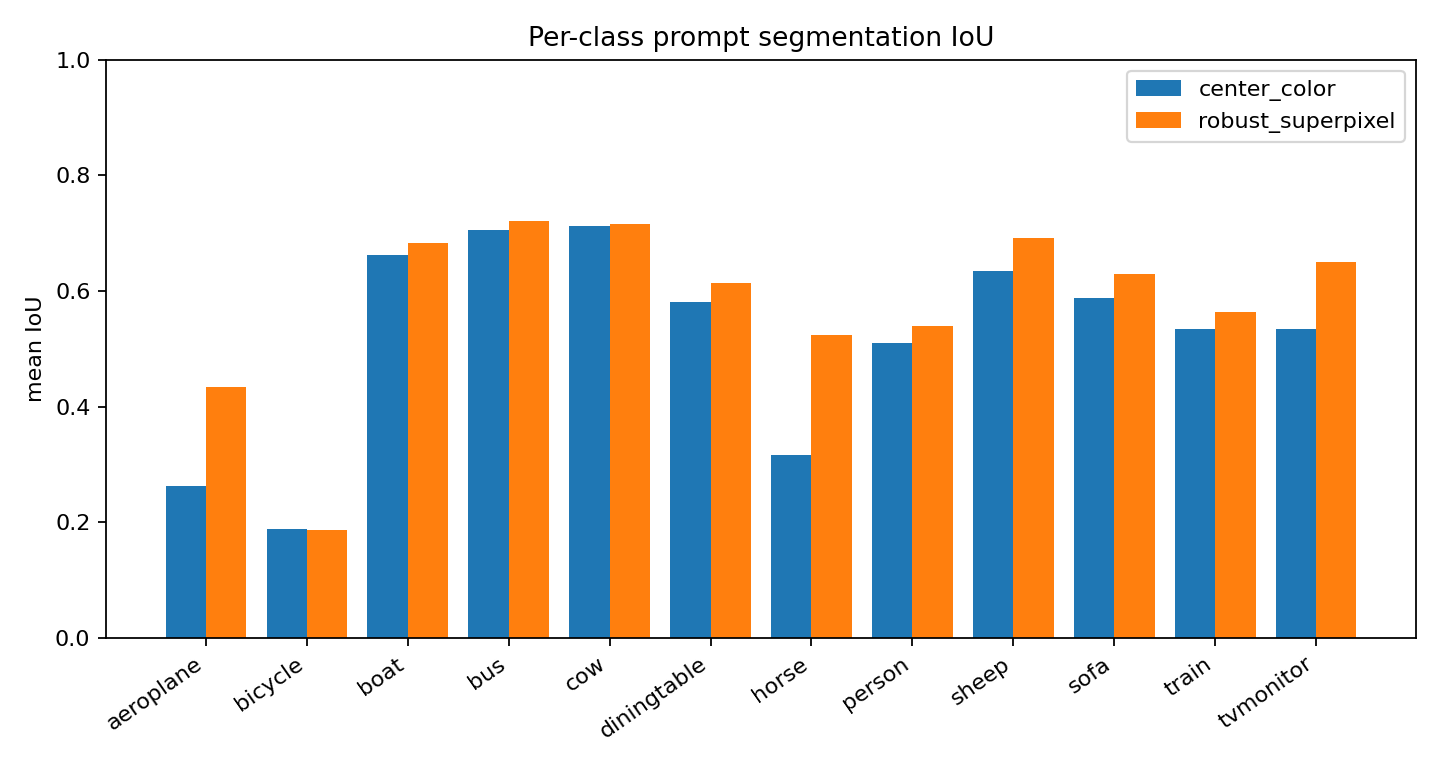
\includegraphics[width=0.86\linewidth]{../outputs/analysis/per_class_iou.png}
\caption{Per-class mean IoU. The strongest gains appear on horse, tvmonitor, and aeroplane examples.}
\end{figure}

\begin{figure}[h]
\centering
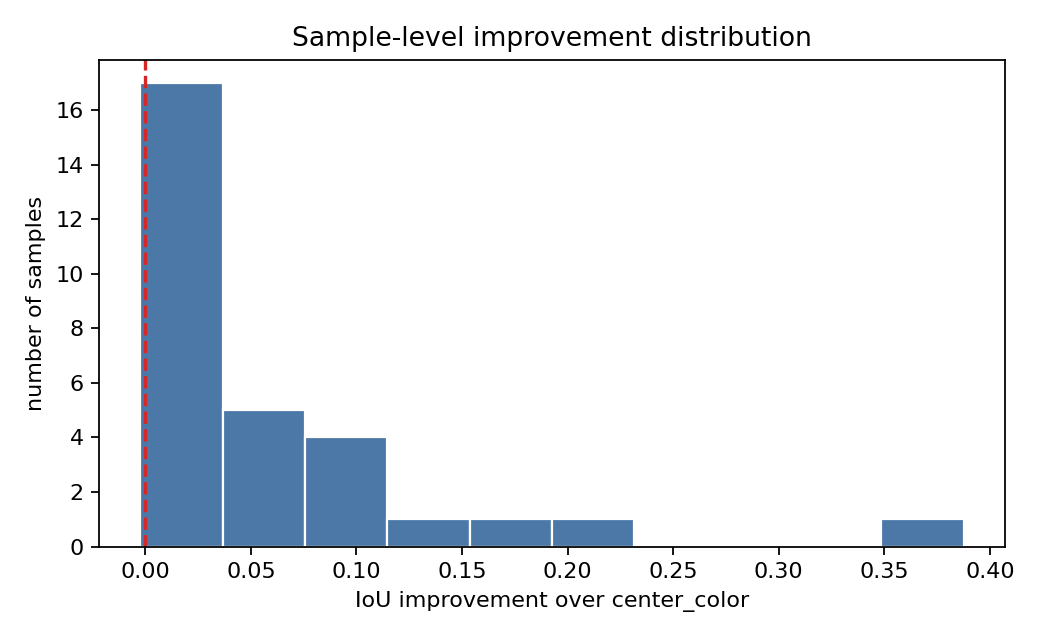
\includegraphics[width=0.68\linewidth]{../outputs/analysis/iou_delta_histogram.png}
\caption{Distribution of sample-level IoU improvement over the center-color baseline.}
\end{figure}

\begin{figure}[h]
\centering
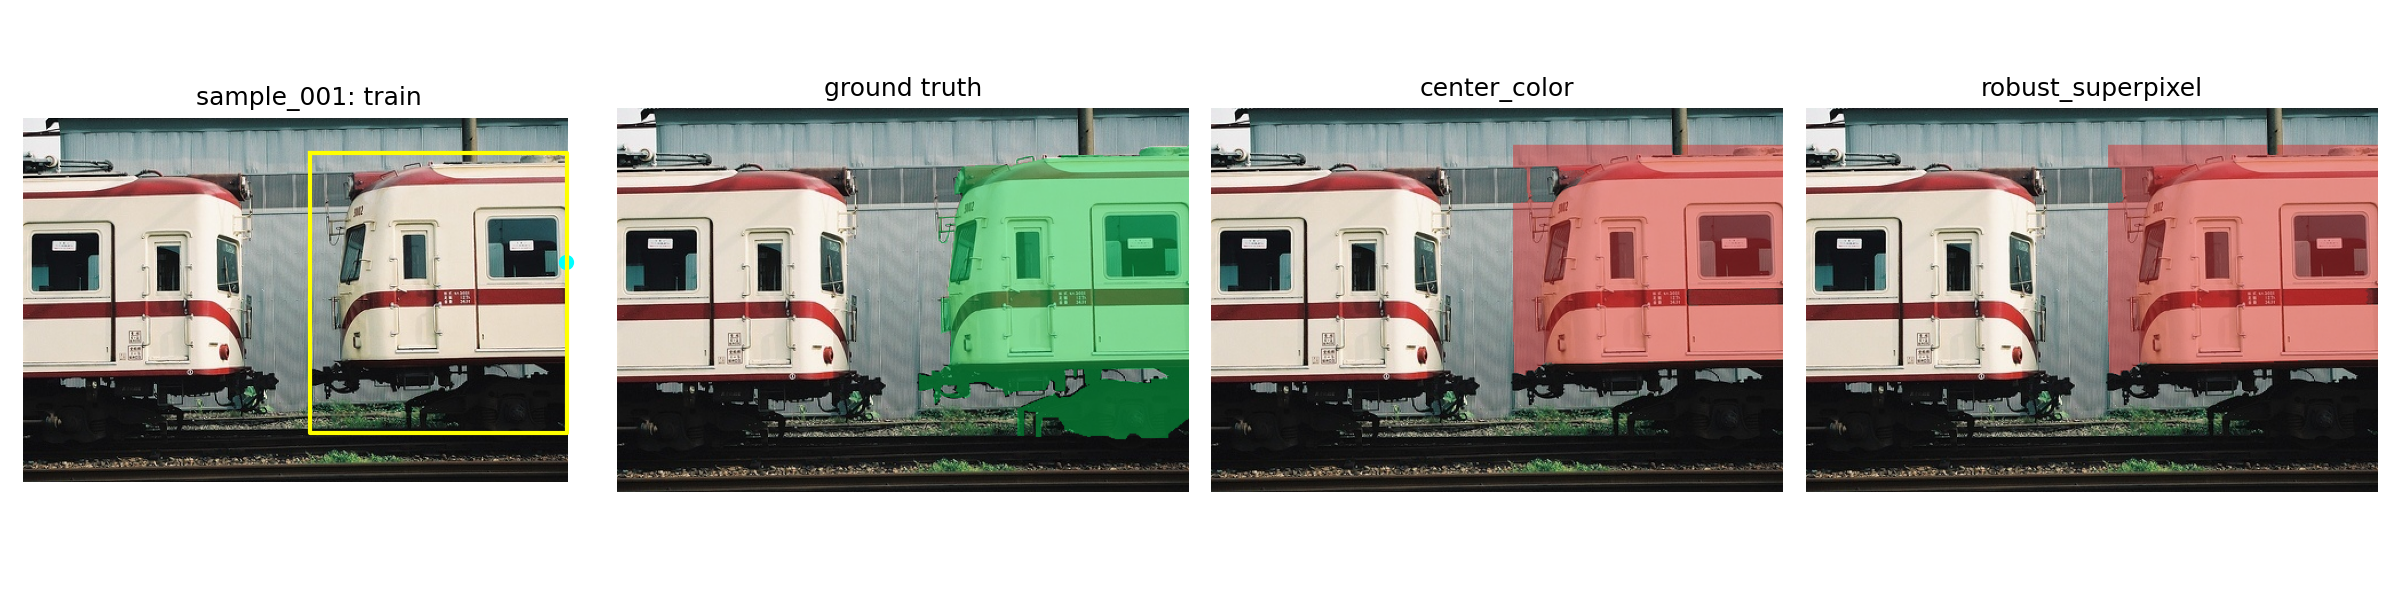
\includegraphics[width=\linewidth]{../outputs/figures/sample_001.png}
\caption{Qualitative example showing prompt, ground truth, center-color prediction, and robust superpixel prediction.}
\end{figure}

\clearpage

\section{Analysis}

The center-color baseline works when the target has a compact appearance and contrasts clearly with the local background. It fails when the object has multiple colors, when the center click lands on a non-representative part, or when background regions share similar colors.

The robust method improves the prompt interface in three ways. First, superpixels better respect local image boundaries than raw pixel thresholding. Second, background evidence from the box boundary and outside-box region suppresses leakage to nearby clutter. Third, box perturbation makes the prediction less sensitive to a single exact prompt.

The hardest cases include train, bicycle, diningtable, and boat images. Trains and dining tables often contain repetitive interior structures, bicycles contain thin parts that are easy to miss, and boats may include strong background colors inside the prompt box. These failures suggest that a SAM-family backend could further improve semantic and boundary understanding.

\section{SAM-Free Baseline and Extension}

PromptLite-Seg is intentionally designed as a SAM-free lightweight baseline. This makes the method CPU-friendly, deterministic, and easy to inspect. In a stronger compute environment, a natural extension is to add a SAM or SAM2 backend using the same point-and-box prompts, then compare SAM predictions with the lightweight baseline and use PromptLite-Seg as a diagnostic fallback.

\section{Conclusion}

This project implements and evaluates a zero-shot prompted segmentation pipeline on PASCAL VOC 2012. It satisfies the course requirement of running an algorithm on a benchmark, and it adds analysis beyond aggregate scores through per-class and success/failure breakdowns. The robust superpixel method provides a transparent and reproducible baseline for prompted segmentation.

\begin{thebibliography}{9}
\bibitem{voc}
Mark Everingham, Luc Van Gool, Christopher K. I. Williams, John Winn, and Andrew Zisserman.
The PASCAL Visual Object Classes Challenge 2012.
\url{https://www.robots.ox.ac.uk/~vgg/projects/pascal/VOC/voc2012/}

\bibitem{sam}
Alexander Kirillov et al.
Segment Anything.
ICCV 2023.
\url{https://arxiv.org/abs/2304.02643}

\bibitem{slic}
Radhakrishna Achanta et al.
SLIC Superpixels Compared to State-of-the-Art Superpixel Methods.
IEEE TPAMI 2012.
\end{thebibliography}

\end{document}
